\chapter*{Aplicação Web}

A primeira decisão a tomar sobre a construção da aplicação web foi em que linguagem o fazer. Depois de analisar algumas hipóteses, escolhemos desenvolver com \textbf{\href{https://angularjs.org/}{AngularJS}}.
\newline Foram necessários um conjunto de passos iniciais para preparar o ambiente para o desenvolvimento:

\begin{enumerate}
    \item npm install http-server -g
    \item http-server -o
\end{enumerate}

E também preparar a estrutura do projeto:

\begin{itemize}
    \item Criar o ficheiro index.html;
    \item Criar a pasta pages e todas as páginas necessárias ao projeto;
    \item Criar o ficheiro app.js, onde se encontra toda a lógica do programa.
\end{itemize}

Posto isto, foi criada uma página para cada tabela da base de dados correspondente e feito o routing no AngularJS. Em cada uma das páginas existe um controller onde é feito o \$http.GET da API da base de dados. Os dados são tratados e visualizados na página html correspondente.
\newline Para a construção de gráficos foi usada a ferramenta \textbf{\href{https://plot.ly/javascript/}{plotlyJS}}.

\begin{figure}[h!]
 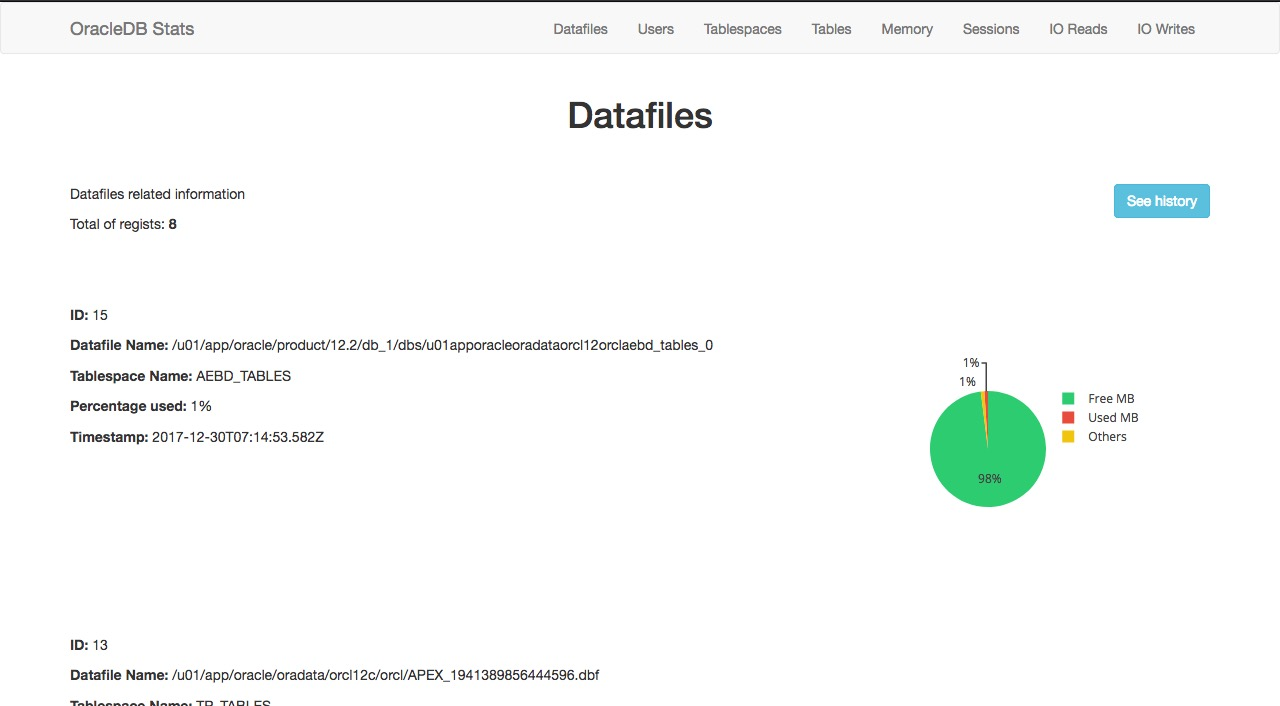
\includegraphics[width=\linewidth]{tex/img/home.jpg}
    \caption{Página correspondente aos Datafiles} 
\end{figure}

\begin{figure}[h!]
 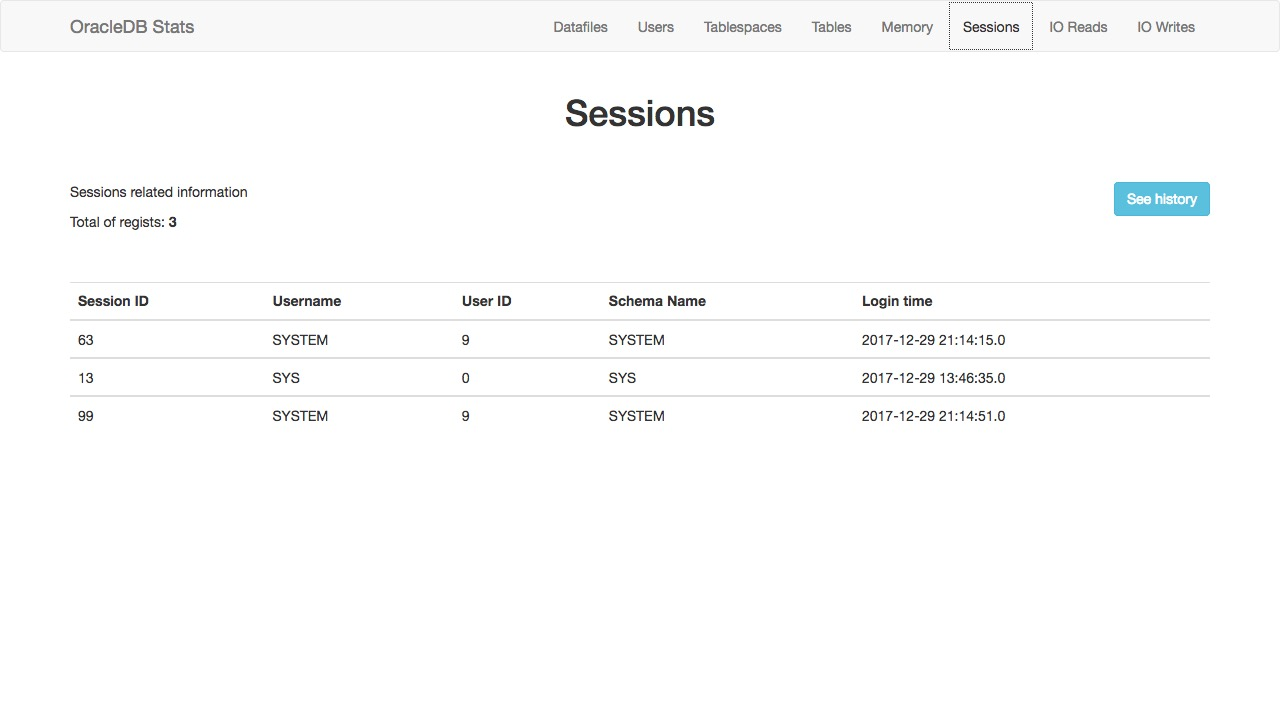
\includegraphics[width=\linewidth]{tex/img/sessions.jpg}
    \caption{Página correspondente às Sessions} 
    \label{fig:esquemarest}
\end{figure}